\chapter{Quaternion}
\label{chap: Quaternion}
In software voor 3D-applicaties wordt eigenlijk niet de rotatie-methode gebruikt zoals die in hoofdstuk \ref{chap: matrix, rotatie en projectie} is beschreven. Vaker wordt de methode van Euler gebruikt, maar die levert problemen op als je over 3 assen roteert. Dat probleem wordt de Gimbal Lock genoemd. Als twee assen over elkaar heen liggen is er een 'vrijheidsgraad' verdwenen en kan een object dus maar in twee richtingen roteren, waar drie richtingen gewenst zijn. Kijk gerust op \href{https://www.youtube.com/watch?v=zjMuIxRvygQ}{\blu{YouTube}} wat info hierover, dit probleem is namelijk makkelijker te snappen met een animatie ervan. Dit is een probleem dat zich zowel in computer graphics als in robotica voor doet. Quaternionen hebben dit probleem niet en worden dan ook veelvuldig ingezet bij rotaties in robotica en computer graphics. Om quaternionen te begrijpen en te kunnen gebruiken moeten we eerst even iets over complexe getallen uitleggen.

\figuur[0.55]{Mandelbrot}{Voorbeeld van een fractal, de Mandelbrotverzameling (Bron: \href{https://en.wikipedia.org/wiki/Mandelbrot_set}{\blu{Wikipedia}}). Tip: Martin Molema kan je over dergelijke figuren van alles vertellen en laten zien. }

\section{Complexe getallen}
Complexe getallen (en quaternionen) zijn zeer handige 'rekenhulpjes' in scala aan werkvelden, zoals in de 3D-simulaties, meet- regeltechniek, signaalbewerking en in de elektrotechniek. Ze zijn daarnaast ook een belangrijk in fractals, daar kun je van die mooie wiskunde figuren uit maken, zoals figuur \ref{fig:Mandelbrot}. 

Complexe getallen zijn een uitbreiding van de reële getallen. Bij het vak discrete wiskunde heb je inmiddels een aantal getalverzamelingen geleerd. bijvoorbeeld $\mathbb{N}$, de natuurlijke getallen. Dit zijn alle gehele getallen vanaf $0$, dus $\mathbb{N} = \{0, 1, 2, 3, \dots\}$. Wil je ook iets doen met negatieve getallen? Bijv. $3-4=?$, Dan is de verzameling $\mathbb{N}$ dus niet toereikend. Je moet dan uitwijken naar een uitbreiding. Bijv. $\mathbb{Z}$, de gehele getallen, deze omvat naast alle getallen van $\mathbb{N}$, ook de negatieve getallen, $\mathbb{Z} = \{\dots, -2, -1, 0, 1, 2, \dots \}$. 

Echter als je $\frac{1}{2} = ?$ wil uitrekenen is ook deze verzameling niet genoeg. Daarvoor kunnen we uitwijken naar de rationele getallen ($\mathbb{Q}$, deze omvat naast alles van $\mathbb{Z}$, ook breuken) of direct naar $\mathbb{R}$, de reële getallen, deze verzameling omvat naast alle getallen van $\mathbb{Q}$ ook bijzondere getallen die niet uit te drukken zijn in een breuk, zoals $\sqrt{2}$ of $\pi$.

\begin{figure}[h!]
    \centering
    \includegraphics[scale=0.35]{pictures/figuren/line.png}
    \caption{$\mathbb{R}$ omvat elk denkbaar getal op een lijn.}
    \label{fig:lijnreeel}
    \index[figuren]{Reële getallen}
\end{figure}

Maar wat nu als je bijv. $x$ probeert op te lossen uit de volgende vergelijking?
\begin{align*}
    x^2 + 1 &= 0 \\
    x^2 &= -1 \\
    x &= \sqrt{-1} \qquad ???
\end{align*}
Er is geen enkel getal in $\mathbb{R}$ waarvan je de wortel kunt nemen zodat er $-1$ uitkomt. Wellicht heb je ooit wel gehoord van een docent wiskunde dat $\sqrt{-1}$ dan ook 'niet kan' en op zich klopt dat, voor $\mathbb{R}$ althans. Maar met complexe getallen is dit wel op te lossen. \mydeftekst[Complexe getallen hebben namelijk een 'imaginair deel', $i$ en daarvoor geldt:]{imaginair }{ 
\[
    i^2 = -1 
\]}

In het bovenstaande voorbeeld zou $x=i$, dus een oplossing zijn. Vaak worden complexe getallen toegepast als er geen (of lastig een) oplossing in $\mathbb{R}$ gevonden kan worden. Men zet dan het getal om in een complex getal, voert daarin allerlei berekeningen uit, en zet het dan weer om naar een reëel getal (Dat laatste gaat in dit kleine voorbeeld echter niet). 

\mydeftekst[We definiëren een complex getal $z$ als:] {getal in $\mathbb{C}$}{ $z=a+bi$ \ met $a$ en $b$ reële getallen}

\mybv[getal in $\mathbb{C}$]{ Bijvoorbeeld, $z=2+3i$ is een complex getal. Complexe getallen ($\mathbb{C}$) kun je zien als $2$-dimensionale getallen, zie ook figuur \ref{fig:lijncomplex}. }
\begin{figure}[h!]
    \centering
    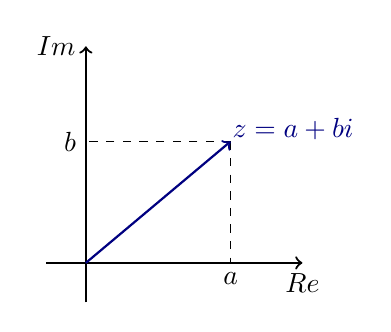
\begin{tikzpicture}
      \def\R{2.4}
      \def\ang{40}
      \coordinate (O) at (0,0);
      \coordinate (X) at (2.75,0);
      \coordinate (Y) at (0,2.75);
      \coordinate (R) at (\ang:\R);
      \coordinate (Rx) at ({\R*cos(\ang)},0);
      \coordinate (Ry) at (0, {\R*sin(\ang)});
      
      % AXIS
      \draw[->,thick] (-0.5,0) -- (X) node[below] {$Re$};
      \draw[->,thick] (0,-0.5) -- (Y) node[left] {$Im$};
      
      % PHASOR
      \draw[dashed] (R) -- (Rx) node[below]{$a$};;
      \draw[dashed] (R) -- (Ry) node[left]{$b$};
      \draw[->, blue!50!black, thick] (O) -- (R) node[above right=-3] {$z=a+bi$};
    \end{tikzpicture}
    
    % \includegraphics[scale=0.15]{pictures/figuren/complex.png}
    \caption{Complexe getallen kun je zien als 2-dimensionaal, waarbij een getal $z$ een 'reëel deel' $a$ heeft en een 'imaginair deel' $bi$.}
    \label{fig:lijncomplex}
    \index[figuren]{Complexe getallen}
\end{figure}

We zeggen ook wel dat $z$ bestaat uit een reëel deel $a$ en een imaginair deel $bi$. Je kunt met complexe getallen net zo rekenen als met reële getallen als je maar rekening houdt met $i^2 = -1$.\mybv[imaginair]{ Bijvoorbeeld:}
\begin{align*}
    (1-i)^2 &= (1-i)\cdot (1-i) \\
            &= (1\cdot 1) + (1\cdot -i) + (-i \cdot 1) + (-i\cdot -i) \\
            &= 1 - i - i -1 \\
            &= -2i 
\end{align*}

\section{Quaternionen}
Quaternionen zijn een uitbreiding van complexe getallen, ze worden aangegeven met $\mathbb{H}$. In plaats van één imaginair deel heb je er hier drie:

\mydeftekst[Een quaternion is:] {quaternion }{\[
  q = a +bi + cj + dk \quad \text{Waarbij: } a, b, c, d \textbf{\textit{ reëel}} \text{ zijn, en } i, j, k 
  \textbf{\textit{ imaginair}}
\]}
Je zou Quaternionen dus kunnen zien als vier-dimensionale getallen, al is dat wat moeilijk grafisch voor te stellen. Bij Quaternionen voldoen $i$, $j$, $k$ zich aan de volgende regels:
\setlength{\abovedisplayskip}{-15pt}
\setlength{\belowdisplayskip}{-5pt}

\begin{align*}
    i^2 &= j^2 = k^2 = i\cdot j\cdot k = -1   \\ & \\
    i\cdot j &= k \qquad \ \ j\cdot i = -k \\
    i\cdot k &= -j \qquad k\cdot i = j \\
    j\cdot k &= i \qquad \ \ k\cdot j = -i      
\end{align*}

\setlength{\abovedisplayskip}{5pt}
\setlength{\belowdisplayskip}{5pt}

Met $a$, $b$, $c$ en $d$ kun je gewoon rekenen, omdat het reële getallen zijn. \mybv[quaternion]{ Ter voorbeeld: $ q_1 = 2 - i  + 2j - 3k $ is een quaternion, net als $ q_2 = - j + k $.}

\subsection{Rekenschema}
Voor het berekenen van de rotatie wordt gebruik gemaakt van quaternion vermenigvuldiging. Twee quaternionen met elkaar vermenigvuldigen gaat via onderstaande tabel:
\begin{center}
	\begin{tabular}{ | l || c | c |c |c |}
		\hline
		& \red{1} & \red{i} & \red{j} & \red{k} \\ \hline \hline
		\blu{1} & 1 & i & j & k \\ \hline
		\blu{i} & i & -1 & k & -j\\ \hline
		\blu{j} & j & -k & -1 & i\\ \hline
		\blu{k} & k & j & -i & -1\\ 
		\hline 
	\end{tabular}
\end{center}

Je zoekt \textit{eerst} in de $ 1^e $ kolom (\blu{blauw} ) welke van $i$, $j$ of $k$ je nodig hebt en \textit{daarna} het volgende  imaginaire getal in de $ 1^e $ rij (\red{rood} ).  Op het kruispunt staat het resultaat van de vermenigvuldiging (de volgorde is belangrijk omdat bijv. $  i\cdot k = -j $ maar $ k\cdot i = j  $ !) 

\mybv[quaterniontabel]{ Als $ q_1 = 6 + 3i - 5j + 2k $ en $ q_2 = 2 + i + 4j - 2k $ wat is dan $ q_1\cdot q_2 $? }
Daarvoor zijn er 2 manieren:

\subsubsection{1. invullen in tabel} Dit is de handigste manier:  Schrijf de eerste quaternion in de eerste kolom en de tweede quaternion in de eerste rij. Vul op de kruispunten de 
vermenigvuldigingen in met de  regels uit het schema. Bijvoorbeeld op het kruispunt van de $ 3^e $ rij en de $   5^e $ kolom: $  3i\cdot -2k = -6ik   $ en omdat $ i\cdot k = -j $ is de uitkomst $ --6j = 6j $. 
\begin{center}
	\begin{NiceTabular}{ | a | c | c | c | c |}
		\hline
        \rowcolor{nhl_blue} \RowStyle{\color{white}} % 
		$ q_1\cdot q_2 $& 2 & i & 4j & -2k \\ \hline 
		6 & 12 & 6i & 24j & -12k  \\ \hline
		3i & 6i & -3 & 12k & 6j\\ \hline
		-5j & -10j &  5k & 20 & 10i\\ \hline
		2k & 4k & 2j & -8i & 4\\ 
		\hline 
	\end{NiceTabular}
\end{center}
Nu kun je het antwoord van linksbovenin tot rechtsonderin af lezen in de tabel. Daarna verzamel je alle $i$, $j$ en $k$:
\begin{align*}
    q_1\cdot q_2 &= 12 + 6i + 24j - 12k + 6i - 3 + 12k + 6j - 10j + 5k + 20 + 10i + 4k + 2j - 8i + 4 \\
                 & = 12 - 3 + 20 + 4 + (6 + 6 + 10 - 8)i +(24 + 6 - 10 + 2)j +(-12 + 12 + 5 + 4)k \\
                 & = 33 + 14i + 22j + 9k
\end{align*}

\newpage
\subsubsection{2. Uitschrijven} Je schrijft alle vermenigvuldigingen op en kijkt per vermenigvuldiging in de tabel wat er uit komt. 'Haakjes wegwerken' dus, weer een flashback naar het vak logica:
\begin{align*}
    q_1\cdot q_2 &= (6 + 3i - 5j + 2k) \cdot  (2 + i + 4j - 2k)& \\
                 &= 6\cdot 2 + 6i + 6\cdot 4j + 6\cdot -2k  &\text{'gewoon' vermenigvuldigen}\\
                 & \ \ \ + 3i\cdot 2 + 3i\cdot i + 3i\cdot 4j + 3i\cdot -2k &i \text{ in } 1^e \text{ kolom opzoeken}\\
                 & \ \ \ + -5j\cdot 2 + -5j\cdot i + -5j\cdot 4j + -5j\cdot -2k  &j \text{ in } 1^e \text{ kolom opzoeken}\\
                 & \ \ \ + 2k\cdot 2 + 2k\cdot i + 2k\cdot 4j + 2k\cdot -2k &k \text{ in } 1^e \text{ kolom opzoeken}\\
                 &= 12 + 6i + 24j - 12k &\\
                 & \ \ \ + 6i - 3 + 12k + 6j &\\
                 & \ \ \ -10j + 5k + 20 + 10i & \\
                 & \ \ \ + 4k + 2j - 8i + 4 \qquad \qquad \qquad   &\text{nu alle } i, j \text{ en } k \text{ bij elkaar  zoeken}\\
                 &= 12 - 3 + 20 + 4 & \\
                 & \ \ \ + (6+ 6 + 10 -8)i & \\
                 & \ \ \ + (24 + 6 - 10 + 2)j & \\
                 & \ \ \ + (-12 + 12 + 5 + 4)k & \\
                 &= 33 + 14i + 22j + 9k & 
\end{align*}
\section{Geconjugeerde quarternion}
Een quaternion kan geconjugeerd worden en dit is ook nodig voor het berekenen van een rotatie. Een geconjugeerde quaternion wordt genoteerd als $q^*$ en wordt in algemene vorm als volgt geschreven:

\mydeftekst{geconjugeerd}{Als $ q = a +bi + cj + dk $  \quad dan is: \quad	$ q^* = a - bi - cj - dk $ }

Let op! Alleen de imaginaire delen $i, j$ en $k$ veranderen van plus naar min (of andersom). Het reële deel ($a$) blijft zoals het is. 

\mybv[geconjugeerd]{ We doen even een paar voorbeeldjes:}
\begin{align*}
  \text{Stel: } q = 1 - 2i + 3j + k &\text{ dan is } q^* = 1 + 2i - 3j - k \\
  \text{En als: } q = i - 3j  &\text{ dan is } q^* = -i + 3j
\end{align*}

\section{Roteren met quaternionen}
We gebruiken quaternionen om te roteren. Daarvoor moeten we dan wel eerst de punten van \RD omzetten naar quaternionen.

\mydeftekst{puntquaternion}{Als $P = (x, y, z)$  in \RD dan is het puntquaternion dat er bij hoort: $p = xi+yj+zk$}

\mybv[puntquaternion]{	Stel: $P = (1, 3, -2)$\ dan is het puntquaternion $p$ dat er bij hoort:}
\[
    p=0 + 1\cdot i+3j-2k\ = i+3j-2k
\]

Voor het berekenen van een rotatie in \RD geldt de volgende formule: \mydeftekst{\small quaternionrotatie}{Als $p$ een punt en $q_r$ een rotatie is in \RD dan is: het geroteerde punt	$p' = q_r\cdot p.q^*_r$ }

\newpage
\setlength{\abovedisplayskip}{5pt}
\setlength{\belowdisplayskip}{5pt}

\mybv[\small quaternionrotatie]{ Bijvoorbeeld:}
Stel $P = (3,0,1)$ en $q_r = 2j-k$ wat is dan $q_r\cdot p\cdot q^*_r $ ?
\begin{align*}
	  p &= 0 + 3i + 0\cdot j + k = 3i+k  \\
	q^*_r &= 0 + 0\cdot i -2j  + k = -2j+k 
\end{align*} 
Dan is de tabel voor $p\cdot q^*_r: $ \quad (p in de $1^e$ kolom, $q^*_r$ in de $1^e$ rij)
	\begin{center}
		\begin{NiceTabular}{ | a | c | c | c | c |}
    		\hline
            \rowcolor{nhl_blue} \RowStyle{\color{white}} %
	$ p\cdot q^*_r $  & 0 & 0 & -2j & k   \\ \hline 
	    		  0 & 0 & 0 & 0   & 0   \\ \hline
                   3i & 0 & 0 & -6k & -3j \\ \hline
                    0 & 0 & 0 & 0   & 0   \\ \hline
                    k & 0 & 0 & 2i  & -1  \\
			\hline 
		\end{NiceTabular}
	\end{center}
En dus is $p\cdot q^*_r = -1+2i-3j-6k$ 
  
Daarna met de tabel  $  q_r\cdot (p\cdot q^*_r) $ uitrekenen  
\quad ($  q_r  $ in de $  1^e $ kolom, $  p\cdot q^*_r: $ in de $ 1^e $ rij)

\begin{center}
	\begin{NiceTabular}{ | a | c | c | c | c |}
		\hline
        \rowcolor{nhl_blue} \RowStyle{\color{white}} %
  $q_r\cdot (p.q^*_r)$ & -1  & 2i  & -3j & -6k  \\ \hline 
                    0  & 0   & 0   &   0 & 0    \\ \hline
                    0  & 0   & 0   &   0 & 0    \\ \hline
                   2j  & -2j & -4k &   6 & -12i \\ \hline
                   -k  & k   & -2j & -3i & -6   \\ 
		\hline 
	\end{NiceTabular}
\end{center}
en dus is $ p' = q_r\cdot (p\cdot q^*_r) =  -15i -4j -3k. $ Dat betekent dat het punt $ P = (3,0,1) $  onder het quaternion  $ q_r = 2j-k $ afgebeeld wordt op het punt $ P' = (-15, -4, -3). $ 

Dat is een vreemde rotatie (want de afstand tot de oorsprong wordt ineens groter). Dat komt omdat we voor $q_r$ wat gemakkelijke waardes hebben genomen en dat is geen echt rotatiequaternion.


Daarom hebben we de volgende definitie nodig: \mydeftekst{\small quaternionrotatie}{Gegeven de eenheidsvector $\hat{v}$ en de  hoek $\alpha $ dan is:	het rotatiequaternion:
\[ 
    q_r = \cos\left(\frac{\alpha}{2}\right) + \sin\left(\frac{\alpha}{2}\right) \hat{v}_1 i + \sin\left(\frac{\alpha}{2}\right) \hat{v}_2 j + \sin\left(\frac{\alpha}{2}\right) \hat{v}_3 k 
\]}

\mybv[\small quaternionrotatie]{ Ter voorbeeld:}
Stel $\vec{v} = \vecdrie{-3}{0}{4} $ dan is $\hat{v} = \frac{1}{5} \vecdrie{-3}{0}{4} $ \quad (omdat $|\vec{v}| = \sqrt{3^2+ 4^2} = 5$)

Stel verder dat we over $\alpha = 180\degree$ willen roteren, dan is $\frac{180\degree}{2} = 90\degree$. We weten dat $  \cos\left(90\degree\right) = 0 $ en  $ \sin\left(90\degree\right) = 1 $ \ \ En dus is: 
\begin{align*}
    q_r &= \cos\left(\frac{180}{2}\right)\ +\ \sin\left(\frac{180}{2}\right) \cdot -\frac{3}{5}\cdot i
           \ +\ \sin\left(\frac{180}{2}\right) \cdot 0\cdot j\ +\ \sin\left(\frac{180}{2}\right) \cdot \frac{4}{5}\cdot k \\
    q_r &= \cos\left(90\right) - \frac{3}{5}\cdot \sin\left(90\right) \cdot i\ +\ \frac{4}{5}\cdot \sin\left(90\right) \cdot k \\
    q_r &= 0 -\frac{3}{5}\cdot 1 \cdot i\ +\ \frac{4}{5}\cdot 1 \cdot k \\
    q_r &= -\frac{3}{5}i + \frac{4}{5}k 
\end{align*}

\mybv[\small quaternionrotatie]{ We nemen dezelfde vector en hoek als hierboven.} Stel verder dat we $P=(-1,-1,0)$ willen roteren. Dan is het puntquaternion $p$:
\[p = -i-j\]
	
We hadden $q_r = -\frac{3}{5}i+\frac{4}{5}k$ en dus is $q^*_r$:
\[
  q^*_r = \frac{3}{5}i - \frac{4}{5}k
\]
	
Eerst moeten we $p\cdot q^*_r$ uitrekenen:
\begin{center}
	\begin{NiceTabular}{ | a | c | c | c | c |}
		\hline
        \rowcolor{nhl_blue} \RowStyle{\color{white}} %
		$ p\cdot q^*_r $  & 0 & $  \nicefrac{3}{5}i  $  & 0 & $ - \nicefrac{4}{5}k $  \\ \hline
		0                 & 0 & 0                       & 0 & 0  \\ \hline
		-i                & 0 &  $  \nicefrac{3}{5}  $  & 0 & $ - \nicefrac{4}{5}j $\\ \hline
		-j                & 0 &  $  \nicefrac{3}{5}k $  & 0 & $  \nicefrac{4}{5}i $\\ \hline
		0                 & 0 & 0                       & 0 & 0 \\
		\hline 
	\end{NiceTabular}
\end{center}

En dus is $p\cdot q^*_r = \frac{3}{5} + \frac{4}{5}i - \frac{4}{5}j + \frac{3}{5}k$

Anders geschreven:
\[
    p\cdot q^*_r = \frac{1}{5}(3 + 4i - 4j  + 3k)
\]

Dit vullen we in in de $1^e$ rij en $q_r$ in de $1^e$ kolom om $q_r\cdot (p\cdot q^*_r)$ te berekenen:
\begin{center}
	\begin{NiceTabular}{ | a | c | c | c | c | l}
		\hline
        \rowcolor{nhl_blue} \RowStyle{\color{white}} %
$ q_r\cdot (p\cdot q^*_r) $  & 3   & 4i  & -4j & 3k  &  $ \times  \frac{1}{5} $\\ \hline
		0                    & 0   & 0   & 0   & 0   & \\ \hline
		-3i                  & -9i & 12  & 12k & 9j  & \\ \hline
		0                    & 0   & 0   & 0   & 0   & \\ \hline
		4k                   & 12k & 16j & 16i & -12 & \\ 
		\hline 
		$ \times  \frac{1}{5} $
	\end{NiceTabular}
\end{center}
Om de berekening overzichtelijk te houden zijn de breuken 'buiten haakjes gehaald'. Zowel voor $q_r$ als voor $p\cdot q^*_r$ is dat $\frac{1}{5}$. 

Dat betekent dat we alles met $\frac{1}{5} \cdot\frac{1}{5} = \frac{1}{25}$ moeten vermenigvuldigen: 
\begin{align*}
    p' &=  q_r\cdot (p\cdot q^*_r)  \\
       &=  \frac{1}{25}(-9i + 12 +12k + 9j + 12k + 16j + 16i - 12) \\
       & = \frac{1}{25} (7i + 25j + 24k)
\end{align*}
En dat betekent dat het punt $ P=(-1,-1,0)  $ waar we mee begonnen  geroteerd wordt naar $P'$:
\[
    P'= \matdrie{\nicefrac{7}{25}}{\nicefrac{25}{25}}{\nicefrac{24}{25}} = \matdrie{0.28}{1}{0.96}  \qquad \text{Zie ook figuur \ref{fig:quatrotatie}}
\]

\figuur[0.6]{quatrotatie}{De rotatie om $\vec{v}$ over $180\degree$. \red{$P(-1,-1,0)$}, wordt geroteerd naar \blu{$P'=(0.28,1,0.96)$}. }

\newpage
\section{Opgaven}
\begin{enumerate}
    \setlength{\itemsep}{10pt}
	\item Gegeven $P (-2, 2, 9)$ en de vector $\vec{v} = \vecdrie{-4}{0}{3} $. 
	We roteren over $84\degree$. Geef het puntquaternion $p$ en het geconjugeerde rotatiequaternion $q_r^*$. 
 
	\item Gegeven $P (23, -15, 7)$ en de vector $\vec{v} = \vecdrie{6}{-6}{7} $. 
	We roteren over $42\degree$. Geef het puntquaternion $p$ en het geconjugeerde rotatiequaternion  $q_r^*$.
	
	\item Gegeven $a = 2i-4j+5k$ en $b = 7+2i+j$. Bereken het product: \ $a\cdot b$
 
	\item Gegeven $c = -16 -2i+3j+2k$ en $d = -1+4i+2k$. Bereken het product: \ $c\cdot d$
 
	\item Gegeven $P (-2, 0, 5)$ en de vector $\vec{v} = \vecdrie{-3}{0}{0} $. 
	We roteren over $60\degree$. Gebruik quaternionen om het beeld van $P$ onder deze rotatie uit te rekenen.
\end{enumerate}

\newpage
\subsection{extra opgaven}
\begin{enumerate}
    \setlength{\itemsep}{10pt}
	\item Gegeven $P (2,2,0)$ en de vector $\vec{v} = \vecdrie{4}{-2}{4} $. 
	We roteren over $42\degree$. Geef het puntquaternion $p$ en het geconjugeerde rotatiequaternion $q_r^*$. 
	
	\item Gegeven $ P (6,-2,3)$ en de vector $\vec{v} = \vecdrie{-12}{12}{6} $. 
	We roteren over $ 84\degree$. Geef het puntquaternion $p$ en het geconjugeerde rotatiequaternion  $q_r^*$. 
	
	\item Gegeven $e = 3 +2j-k$ en $f = 2i+3j+3k$. Bereken het product: \ $e\cdot f$
	
	\item  Gegeven $P (-2, 0, 0)$ en de vector $\vec{v} = \vecdrie{0}{7}{0} $. 
	We roteren over $60\degree$. Gebruik quaternionen om het beeld van $P$ onder deze rotatie uit te rekenen. 
	
	\item Schrijf een programma dat quaternionen kan vermenigvuldigen.  
	
	\item Schrijf een programma dat quaternionrotatie kan uitvoeren (dus gegeven een willekeurige vector $\vec{v}$, hoek $\alpha$ en punt $P$, kan uitrekenen waar $P'$ onder de rotatie uitkomt).  
\end{enumerate}
